\documentclass [a4paper] {article}
\usepackage[utf8]{inputenc}
\title{Ciencia de datos, práctica 2}
\author{Juan Casado Ballesteros, Samuel García Gonzalez, Iván Anaya Martín}
\usepackage{Sweave}
\begin{document}
\maketitle

\begin{abstract}

\end{abstract}

\newpage
\tableofcontents
\newpage


\section{EJ1}

\section{EJ2}
Creamos un .txt con los datos proporcionados sobre el radio y densidad de los planetas y lo leemos.
\begin{Schunk}
\begin{Sinput}
> datos2 <- read.table("datos2.txt")
> datos2
\end{Sinput}
\begin{Soutput}
    Nombre Radio Densidad
1 Mercurio   2.4      5.4
2    Venus   6.1      5.2
3   Tierra   6.4      5.5
4    Marte   3.4      3.9
\end{Soutput}
\end{Schunk}

Calculamos la regresión sobre dichos datos para obtener la recta que más se aproxime a los puntos que tenemos.
\begin{Schunk}
\begin{Sinput}
> regresion2 <- lm(Densidad~Radio, data=datos2)
\end{Sinput}
\end{Schunk}

Podemos ver los valores que adopta la ecucaión de la recta que se generará.
\begin{Schunk}
\begin{Sinput}
> # y = ax + b
> regresion2$coefficients[1] # b
\end{Sinput}
\begin{Soutput}
(Intercept) 
   4.362396 
\end{Soutput}
\begin{Sinput}
> regresion2$coefficients[2] # a
\end{Sinput}
\begin{Soutput}
    Radio 
0.1393669 
\end{Soutput}
\end{Schunk}

Cuando calculamos la recta de regresión sobre unos datos es necesario evaluar la calidad de esta.
Debemos analizar cómo de bien se ajusta a nuestros datos.
Podemos ver esta información mediante summary.

\subsection{Residuos}
Diferencias entre cada valor de y real y cada valor de y obtenido mediante la función de regresión.
\begin{Schunk}
\begin{Sinput}
> summary(regresion2)$residuals
\end{Sinput}
\begin{Soutput}
          1           2           3           4 
 0.70312301 -0.01253452  0.24565541 -0.93624389 
\end{Soutput}
\end{Schunk}

\subsection{Coeficientes}
Coeficientes estimados para y error estándar para cada uno de ellos.
\begin{Schunk}
\begin{Sinput}
> summary(regresion2)$coefficients
\end{Sinput}
\begin{Soutput}
             Estimate Std. Error   t value   Pr(>|t|)
(Intercept) 4.3623964  1.2049754 3.6203201 0.06854492
Radio       0.1393669  0.2466205 0.5651067 0.62893696
\end{Soutput}
\end{Schunk}

\subsection{Error estándar}
Podemos comprobar que coincide con nuestra implementación.
Cuanto más próximo a 0 sea el error estándar mejor será la recta de regresión.
\begin{Schunk}
\begin{Sinput}
> summary(regresion2)$sigma
\end{Sinput}
\begin{Soutput}
[1] 0.8460019
\end{Soutput}
\begin{Sinput}
> errorEstandar(datos2$Radio, datos2$Densidad, regresion2)
\end{Sinput}
\begin{Soutput}
    Radio 
0.8460019 
\end{Soutput}
\end{Schunk}

\subsection{Correlación cuadrada}
Podemos comprobar que coincide con nuestra implementación.
Este valor está entre 0 y 1 siendo mejor cuanto más próximo a 1 sea (idealmente a partir de 0.8).
\begin{Schunk}
\begin{Sinput}
> summary(regresion2)$r.squared
\end{Sinput}
\begin{Soutput}
[1] 0.1376878
\end{Soutput}
\begin{Sinput}
> correlacionCuadrada(datos2$Radio, datos2$Densidad)
\end{Sinput}
\begin{Soutput}
    Radio 
0.1376878 
\end{Soutput}
\end{Schunk}

Para finalizar dibujaremos una gráfica en la que se representarán lod datos junto a la recta de regresión.
Paralela a la recta de regresión dibujaremos las rectas que marcan el error estándar entorno a la recta de regresión.
En trazado gris grueso la que marca la región en la que estarán el 66\% de los datos y en gris fino la que marca el 95\%.
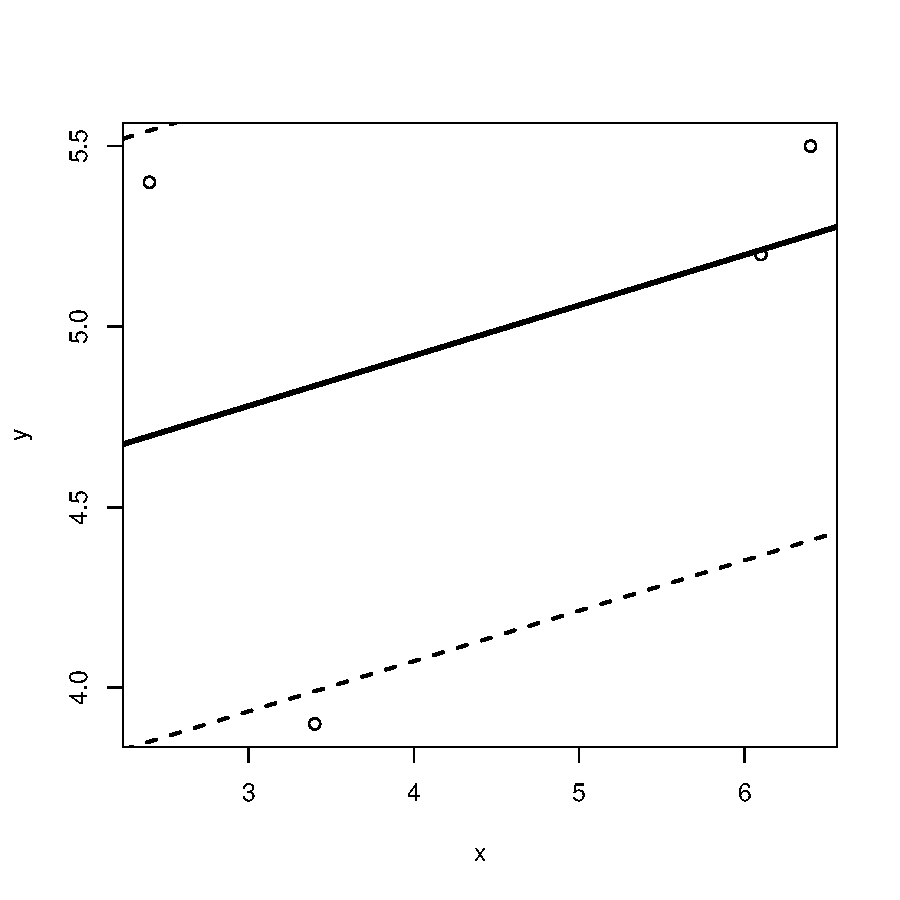
\includegraphics{entrega2-plot_regresion2}


\section{EJ3}




\end{document}
